\chapter{Background and Related Work} % (fold)
\label{cha:Related_Work}
\section{Twitter}
Twitter is a mircoblogging service. Now there are more than 140 million active users\footnote{https://blog.Twitter.com/2012/Twitter-turns-six}. User can publish short messages within 140 characters aka tweets.
\subsection{Retweet}
A retweet is re-posting of a tweet by other users. One way of retweet is using RT at the beginning of the tweet which is retweeted. The other way is using "retweet button" which is officially launched by Twitter after 2015. The difference between these two retweet is tweets are retweeted by "retweet button" can't be searched by Twitter's searching interface, but manually retweets with RT keyword can. So in our work retweet means the tweets are retweeted manually. The number of how many times of this tweet has been retweeted is showed behind it.

\subsection{Mentions}
Mentions are in form like "@username" which are added in the text of tweet. The users are mentioned will receive the notification of this tweet on their homepage.
\subsection{Hashtags}
Mentions are in form like "\#topic". It means this tweet belongs to some topics.

\subsection{Favorite}
Favorites means how many users like this tweet. It is showed on the interface of Twitter
\subsection{Verified User}
Verified User means this account of public interest is authentic by Twitter. It is showed by a blue icon behind the name of the poster.
\subsection{Followers}
The followers of a user are accounts who receive this user's posting. The total number of followers can been seen in the profile of poster.
\subsection{Following}
The following are other accounts who follow this user. The total number of following can been seen in the profile of poster.
\subsection{Twitter API}
\label{tapi}
Twitter API is provided by Twitter\footnote{https://dev.twitter.com/overview/api} for developer. But the search API only return a sampling of recent Tweets published in the past 7 days\footnote{https://dev.twitter.com/rest/public/search}. We need the full stories of the events, so we crawled the data directly from the searching interface\footnote{https://twitter.com/search-home}.
\section{Credibility of Tweets } % (fold)
Titter has been used for reporting breaking news when emergency events happen like disaster \cite{kwak2010twitter}. But the people are likely to trust the news which post on traditional news website more than the news with same headline but posted on twitter\cite{java2007we}. And Thomson's work shows that different crowds of people trust tweets basing on different kinds of sources \cite{thomson2012trusting}.
 \section{Definition of Rumor}
 The definition of rumor in our work is unverified information spreading on Twitter over time. It is a set of tweets including the the sources, spreaders, retweets, doubting  tweets and the denying tweet. 
 \subsection{Rumor Event}
 If a rumor didn't widely spread and it could be harmless. So we more focused on the rumors which are widely spread and contain one or more bursty pikes during propagation. We call it "rumor event".
\subsection{Time Period of an Event}
\label{sec:Time_Period_of_an_Event}

The beginning of a rumor event is hard to define. As far as I  know there is related work which give us a approach to define the beginning of one rumor event. One reason is a rumor may be created serval years ago and kept exiting in Twitter, but it didn't attract the people's attention. However it can be triggered by other events and suddenly quickly spread as a bursty event.

For example, a rumor\footnote{http://www.snopes.com/robert-byrd-kkk-photo/} claimed that Robert Byrd was member of KKK. This rumor has been circulating in Internet for a while, as shown in figure \ref{fig:KKK_full} that almost every day there are several tweets talking about this rumor. But this rumor was triggered by a picture about Robert Byrd kissing Hillary Clinton in 2016 and twitter users suddenly notice this rumor and this rumor was bursty spread. So what we are really interested in is the hours around the bursty pike.
 
\begin{figure}[!h]
\centering
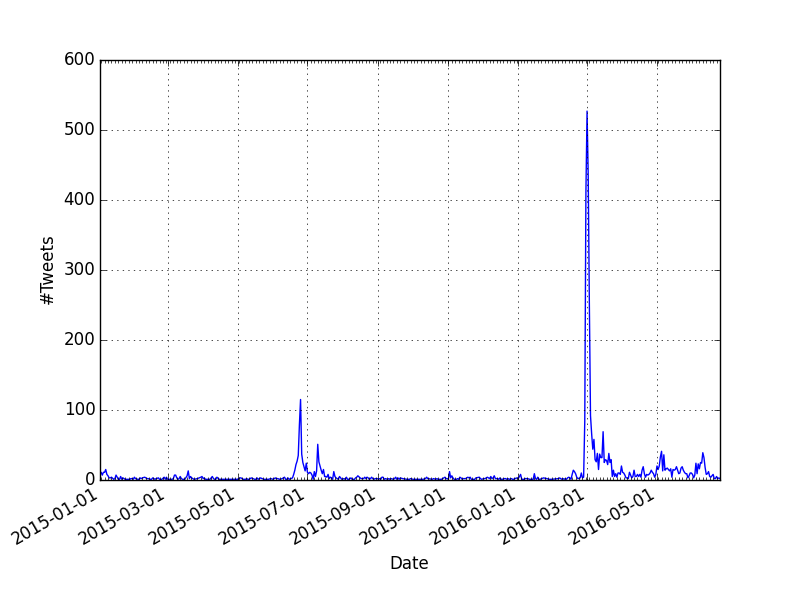
\includegraphics[width=0.7\columnwidth]{images/KKK_figure.png}
\caption{large scale tweet volume of event Robert Byrd}
\label{fig:KKK_full}
\end{figure}

 We defined the hour which has the most tweet's volume as $t_{max}$ and we want to detect the rumor event as soon as possible before its burst, so we define the time of the first tweet before $t_{max}$ within 48 hours as the beginning of this rumor event, marked as $t_{0}$. And the end time of events we defined as $t_{end}=t_0+48$. We show the tweet volume in figure \ref{fig:KKK_part} of the above rumor events after defined 48 hours time period.
  
\begin{figure}[!h]
\centering
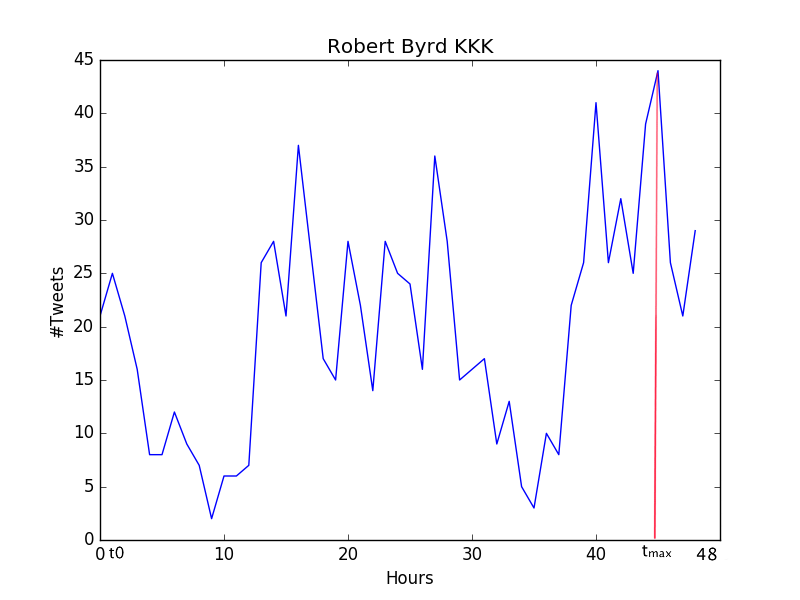
\includegraphics[width=0.7\columnwidth]{images/Robert_Byrd_KKK.png}
\caption{tweet volume of the rumor event of Robert Byrd after selected time period}
\label{fig:KKK_part}
\end{figure}



\section{Machine Learning } % (fold)
\label{sec:Maschine_learning}
\subsection{Machine learning Overview} % (fold)

% Why are archives valuable
 Machine learning covers vast numbers of algorithms and has been successful applied in different field. The challenges of ML are finding the best model which is suitable for this task, fitting the parameters and selecting the features. 
 
Normally we split the ML methods into Supervised learning, Unsupervised learning and Reinforcement learning\cite{russell2003artificial}. 

The supervised learning is the most popular method of ML. It needs a set of inputs and a set of desired outputs. And the algorithm will learn to produce the correct output based on the new input. 

The unsupervised learning needs a set of inputs but no outputs. The algorithm will generate the outputs like clusters or patterns. The unsupervised learning task can be used for example when people can't label the outputs. 
\subsection{ Decision Tree} % (fold)
Classification is a supervised data mining technique. Our work can be considered as a classification task. Decision tree is a model we use for base line in the after work. A decision tree uses a tree model of decisions and their possible consequences as shown in figure \ref{fig:detrees}.  DT is an non-parametric supervised learning method used for classification and regression. Because the trees structure is very simple to visualize, the result of DT is easy to understand. But Decision trees are unstable \cite{breiman1996bagging}. But DT is the basic unit of random forest.
\begin{figure}[!h]
\center
\tikzset{
 sibling distance={6em},
  treenode/.style = {shape=rectangle, rounded corners,
                     draw, align=center,
                     top color=white, bottom color=blue!20},
  root/.style     = {treenode, font=\Large, bottom color=red!30},
  env/.style      = {treenode, font=\ttfamily\normalsize},
  dummy/.style    = {circle,draw},
      level distance          = 10em,
   edge from parent/.style = {draw, -latex}
}

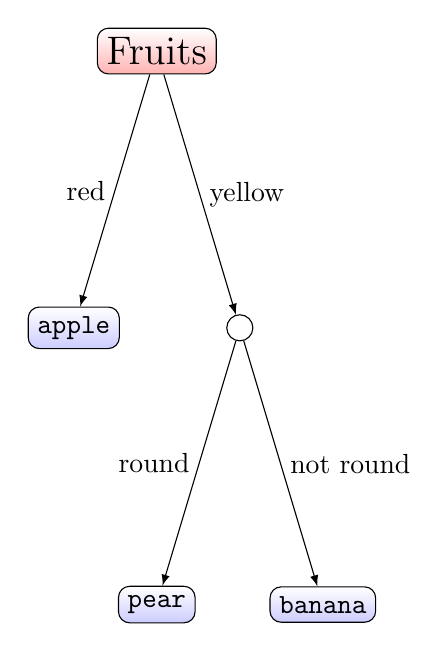
\begin{tikzpicture}
  
\node [root] {Fruits}
    child { node [env]{apple} edge from parent node [left] {red}}
    child { node [dummy] {}
      child { node [env] {pear} edge from parent node [left] {round}
      }
      child { node [env] {banana} edge from parent node [right] {not round}
      } edge from parent node [right] {yellow}
       };
\end{tikzpicture}
\caption{Decision tree}
\label{fig:detrees}

\end{figure}

\subsection{Random Forest (RF)} % (fold)
\label{random_forest}
 Another we use for testing is random forest.

RF is an algorithm of supervised learning which developed by Leo Breiman \cite{breiman2001random}. It's built by a set of classification trees \cite{breiman1984classification}. Each tree is trained by a small bootstrap sample of training set and while prediction each tree votes one single candidate. RF generates the result of prediction By taking the majority vote. 

For example we got task to classify pears and apples. We have the features are whether the fruit round, whether the fruit has seeds, whether the fruit red and whether the fruit is juicy. We build up a 3 trees random forest as the graph \ref{fig:randomforest}. Tree 1 randomly takes the subset of the features red and seeds and votes to apple. Tree 2 randomly takes the subset of the features red and seeds and votes to pear. Tree 3 randomly takes the subset of the features round and red and votes to apple. The most vote is apple, so the output of RF is apple.

\begin{figure}[!h]
\tikzset{
 sibling distance={6em},
  treenode/.style = {shape=rectangle, rounded corners,
                     draw, align=center,
                     top color=white, bottom color=blue!20},
  root/.style     = {treenode, font=\Large, bottom color=red!30},
  env/.style      = {treenode, font=\ttfamily\normalsize},
  dummy/.style    = {circle,draw},
      level distance          = 10em,
   edge from parent/.style = {draw, -latex}
}

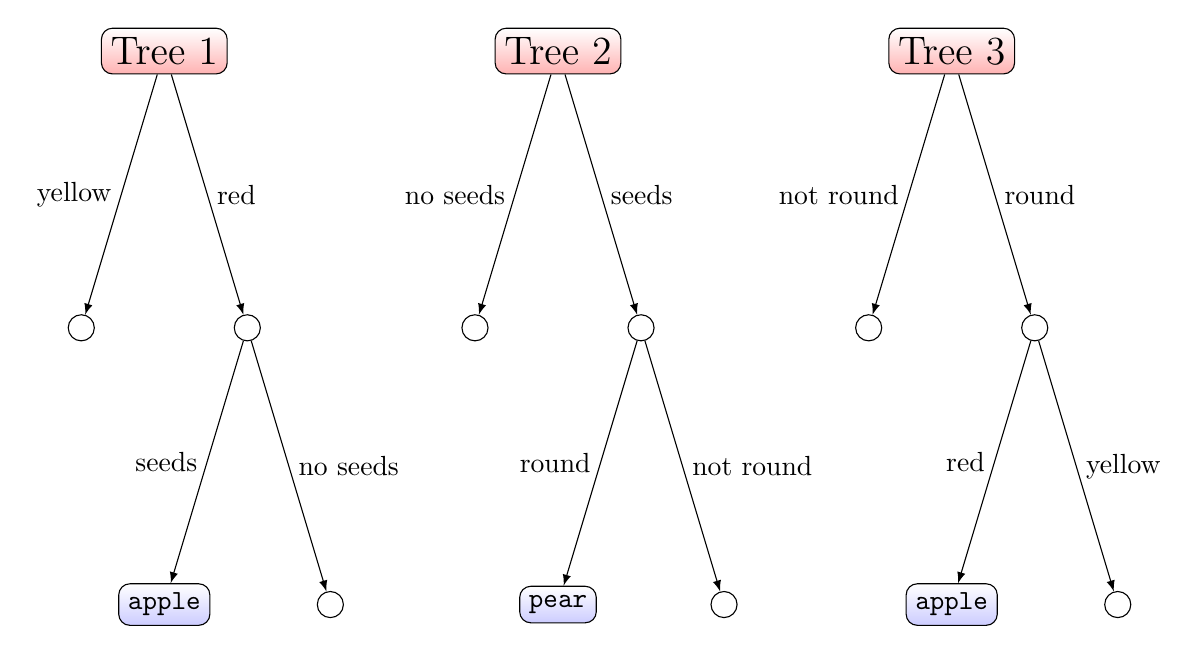
\begin{tikzpicture}
 \begin{scope} 
\node [root] {Tree 1}
      child { node [dummy] {} edge from parent node [left] {yellow}}
    child { node [dummy] {}
      child { node [env] {apple} edge from parent node [left] {seeds}
      }
      child { node [dummy] {} edge from parent node [right] {no  seeds}
      } edge from parent node [right] {red}
       };
       
       \end{scope}

  \begin{scope}[xshift=5cm]
\node [root] {Tree 2}
    child { node [dummy] {} edge from parent node [left] {no  seeds}}
    child { node [dummy] {}
      child { node [env] {pear} edge from parent node [left] {round}
      }
      child { node [dummy] {} edge from parent node [right] {not round}
      } edge from parent node [right] {seeds}
       };
  \end{scope}
  \begin{scope}[xshift=10cm]
\node [root] {Tree 3}
     child { node [dummy] {} edge from parent node [left] {not   round}}
    child { node [dummy] {}
      child { node [env] {apple} edge from parent node [left] {red}
      }
      child { node [dummy] {} edge from parent node [right] {yellow}
      } edge from parent node [right] {round}
       };
  \end{scope}
\end{tikzpicture}
  \caption{An example of random forest with 3 trees}
\label{fig:randomforest}
\end{figure}


Because RF uses a random subset of features instead of the best features in every node, so it can avoid the overfitting problem \cite{breiman2001random}. 

Another benefit of RF is that it can return the \textbf{features' importance}. RF is built up by a subset of training data. If there are N trees, RF will take N times bootstrap sampling. So some features we didn't select to use for training the model. The data we didn't selected we call it out-of-bag (OOB) data. In the above example the feature whether the fruit is juicy didn't join the construction the Trees, so it is a OOB data. These data can be use for validating the model and the output is OBB error $E_{oob}(G) = \frac {1}{N} \sum_{n=1}^{N}err(y_n,G_{n}^-(X_n))$ with $X_n$ are features only in OOB. At last we get the importance of feature by permuting one feature to random numbers. $importance(i)= E_{oob}(G)-E_{oob}^{p}(G)$; where $E_{oob}^{p}(G)$ is the OBB error after permuting a feature. The more performance drop down, that means the more important this feature is. We use this method to measure the performance of features and evolute the models later. 
One more important benefit of RF is it can easily visualize, so it can convince people not only by the test accuracy  but also by the giving us a good explanation, for example rumor containing more negative sentiment or the poster of real news more likely living in large city. 


\section{Neural Network} % (fold)
Figure \ref{fig:NN} is a simple model of forwarding neural network which is a computing systems that processes information by their dynamic state response to external inputs [39]. In the figure  \ref{fig:NN}  
the round nodes are called neurons. Each neuron has a active function like sigmod or tanh \ref{fig:tanh} Neurons are connected each others with weight. The process of training the model is actually the process learning the weights of the connections of the network. With the back-propagation algorithm we 1) compute the loss from the network
output and 2) update the weights by passing the error
backwards through the network \cite{rumelhart1988learning}.  
\begin{figure}[!h]
\center
\def\layersep{2.5cm}

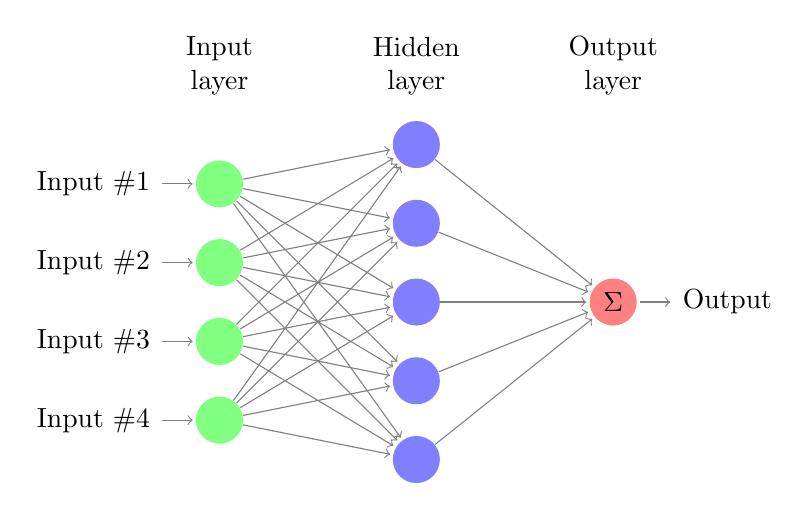
\begin{tikzpicture}[shorten >=1pt,->,draw=black!50, node distance=\layersep]
    \tikzstyle{every pin edge}=[<-,shorten <=1pt]
    \tikzstyle{neuron}=[circle,fill=black!25,minimum size=17pt,inner sep=0pt]
    \tikzstyle{input neuron}=[neuron, fill=green!50];
    \tikzstyle{output neuron}=[neuron, fill=red!50];
    \tikzstyle{hidden neuron}=[neuron, fill=blue!50];
    \tikzstyle{annot} = [text width=4em, text centered]

    % Draw the input layer nodes
    \foreach \name / \y in {1,...,4}
    % This is the same as writing \foreach \name / \y in {1/1,2/2,3/3,4/4}
        \node[input neuron, pin=left:Input \#\y] (I-\name) at (0,-\y) {};

    % Draw the hidden layer nodes
    \foreach \name / \y in {1,...,5}
        \path[yshift=0.5cm]
            node[hidden neuron] (H-\name) at (\layersep,-\y cm) {};

    % Draw the output layer node
    \node[output neuron,pin={[pin edge={->}]right:Output}, right of=H-3] (O)  {$\displaystyle\Sigma$};

    % Connect every node in the input layer with every node in the
    % hidden layer.
 
    \foreach \source in {1,...,4}
        \foreach \dest in {1,...,5}
            \path (I-\source) edge (H-\dest);

    % Connect every node in the hidden layer with the output layer
    \foreach \source in {1,...,5}
        \path (H-\source) edge (O);

    % Annotate the layers
    \node[annot,above of=H-1, node distance=1cm] (hl) {Hidden layer};
    \node[annot,left of=hl] {Input layer};
    \node[annot,right of=hl] {Output layer};
\end{tikzpicture}

   \caption{An example of 1 layer neural network}
\label{fig:NN}
\end{figure}
\label{sec:NNsec}

 \begin{figure}[h]
\center
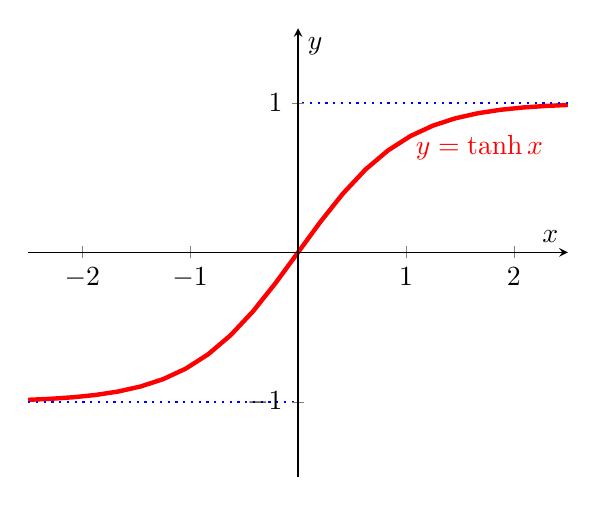
\begin{tikzpicture}
\begin{axis}[
    xmin=-2.5, xmax=2.5,
    ymin=-1.5, ymax=1.5,
    axis lines=center,
    axis on top=true,
    domain=-2.5:2.5,
    ylabel=$y$,
    xlabel=$x$,
    ]

    \addplot [mark=none,draw=red,ultra thick] {tanh(\x)};
    \node [right, red] at (axis cs: 1,0.7) {$y = \tanh x$};

    %% Add the asymptotes
    \draw [blue, dotted, thick] (axis cs:-2.5,-1)-- (axis cs:0,-1);
    \draw [blue, dotted, thick] (axis cs:+2.5,+1)-- (axis cs:0,+1);
\end{axis}
\end{tikzpicture}
   \caption{tanh function}
\label{fig:tanh}
\end{figure}
\newpage
 \subsection{Convolutional Neural Network} % (fold)
CNN is a kind of neural network which contains a convolutional layers. First CNN is developed by LeCun et al. developed CNNs \cite{lecun1989backpropagation} for computer vision to resolve the problem of imagines' shift or rotation. With the convolutional layer CNN make that is possible to learn from the local features. Figure \ref{fig:cnn2} is an example p of CNN in application of text classification. The word "wait" and its following word "for" are mapped together into different classes though different convolutional filters. That makes convolutional neural network does not learn from the single word form sentence but from the word and its context. That makes sense because one word can in different context have different meaning. For example "Apple Tree" and "Apple Company", the same apple but contains different meaning. 
 Pooling layer often follows after the convolutional layers in CNN models whose mainly task is to down-sample from the output of convolutional layers.  
 
 We use it for for single tweet's creditability score model in the later section \ref{sec:single_nofeature}
   


 \begin{figure}[!h]
\centering
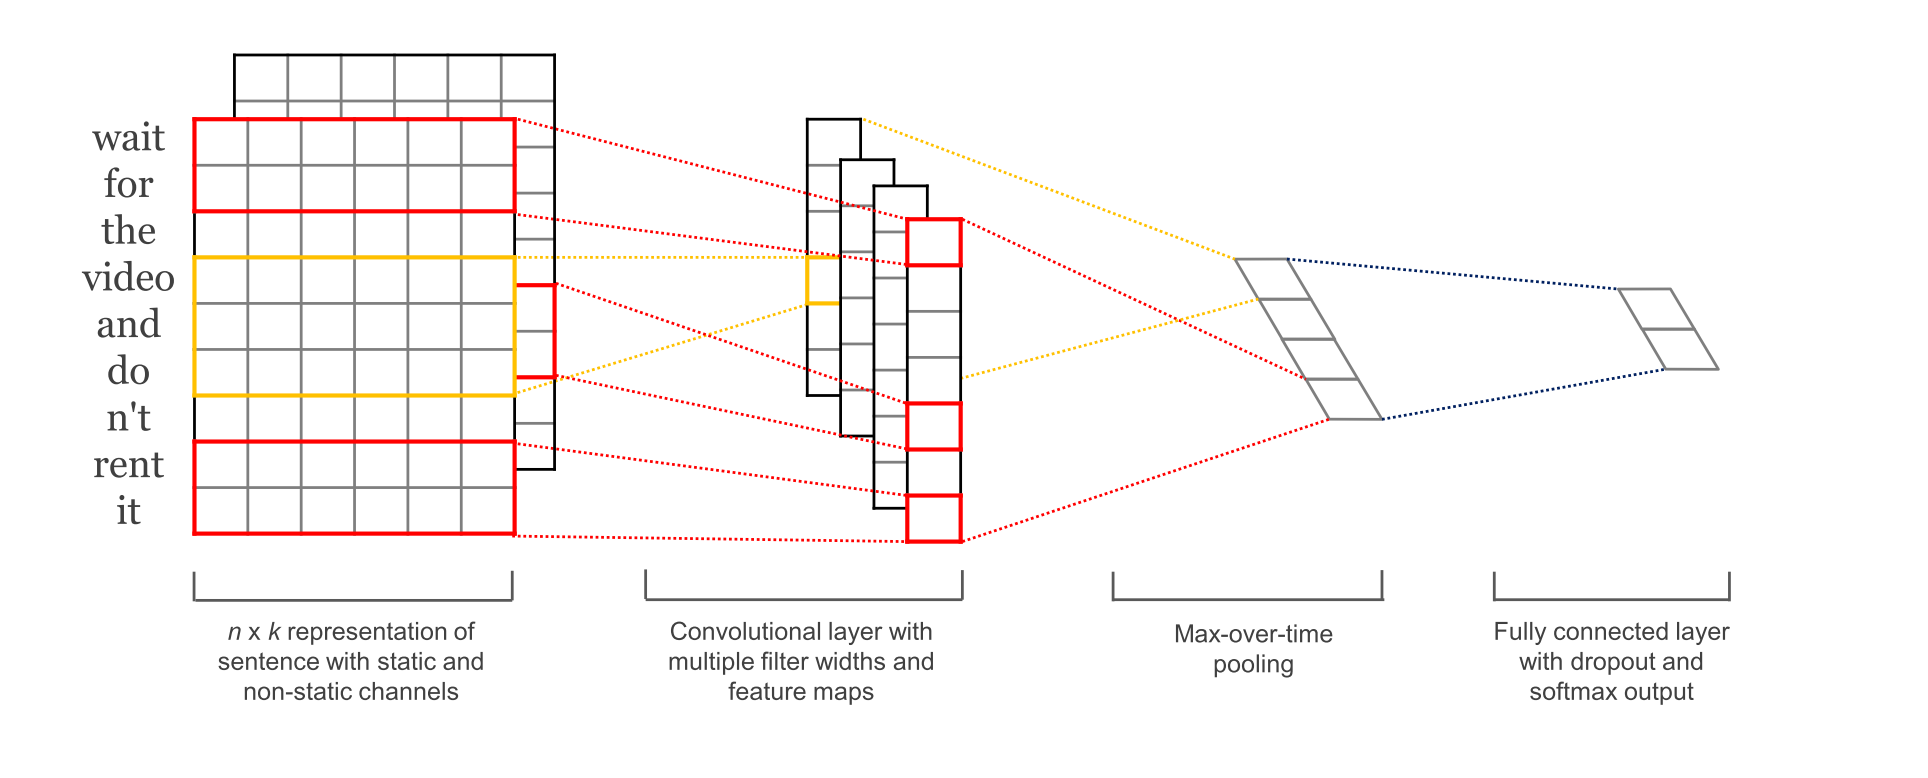
\includegraphics[width=1\columnwidth]{images/CNN.png}
\caption{CNN for Text Classification (source from\cite{kim2014convolutional}) }
\label{fig:cnn2}
\end{figure}



\subsection{Recurrent Neural Network} % (fold)

A Recurrent neural network (RNN) is one of of class of neural network. The different between RNN and other neural network is there are feedback connections between the hidden layers showing as figure \ref{fig:RNNfull}, that makes the input from the past also can influence the network. The activation status of the hidden layer neurons presents as an internal state which can be considered as a kind of memory. That makes recurrent neural network has the ability to process the sequence input. Human understand the words of a sentence often need the help of the previous words, but the feed forwarding neural network will ignore the previous inputs.


\begin{figure}[!h]
\center
\def\layersep{1.8cm}

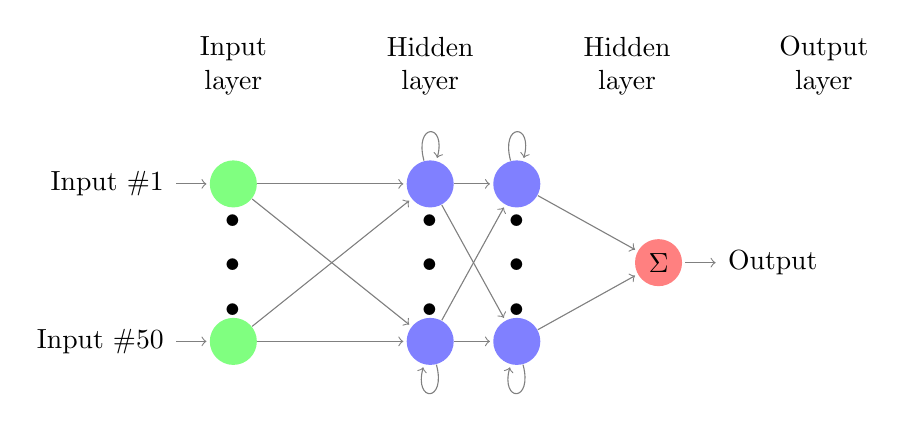
\begin{tikzpicture}[shorten >=1pt,->,draw=black!50, node distance=\layersep]
    \tikzstyle{every pin edge}=[<-,shorten <=1pt]
    \tikzstyle{neuron}=[circle,fill=black!25,minimum size=17pt,inner sep=0pt]
    \tikzstyle{input neuron}=[neuron, fill=green!50];
    \tikzstyle{output neuron}=[neuron, fill=red!50];
    \tikzstyle{hidden neuron}=[neuron, fill=blue!50];
    \tikzstyle{annot} = [text width=4em, text centered]
    \tikzstyle{neuron missing} = [draw=none,scale=4,text height=0.333cm , execute at begin node=\color{black}$\vdots$]
    % Draw the input layer nodes
     % This is the same as writing \foreach \name / \y in {1/1,2/2,3/3,4/4}
        \node[input neuron, pin=left:Input \#1] (I-1) at (0,-1) {};
        \node[input neuron, pin=left:Input \#50] (I-2) at (0,-3) {};
        \node[neuron missing,]  at (0,-2) {};

    % Draw the hidden layer nodes
         \node[hidden neuron] (H-2) at (\layersep,-3) {};
         \node[hidden neuron] (H-1) at (\layersep,-1) {};
        \node[neuron missing,]  at (\layersep,-2) {};
        
         \node[hidden neuron] (W-2) at (3.6,-3) {};
         \node[hidden neuron] (W-1) at (3.6,-1) {};
        \node[neuron missing,]  at (3.6,-2) {};

    % Draw the output layer node
    \node[ output neuron,pin={[pin edge={->}]right:Output},  xshift=5.4cm,yshift=-2cm] (O) {$\displaystyle\Sigma$};

    % Connect every node in the input layer with every node in the
    % hidden layer.
 
    \foreach \source in {1,...,2}
        \foreach \dest in {1,...,2}
            \path (I-\source) edge (H-\dest);
    \foreach \source in {1,...,2}
        \foreach \dest in {1,...,2}
            \path (H-\source) edge (W-\dest);
     \path  (W-1) edge [loop above]  (W-1);
     \path  (W-2) edge [loop below]  (W-2);


     % Connect every node in the hidden layer with the output layer
    \foreach \source in {1,...,2}
        \path (W-\source) edge (O);
       
     \path  (H-1) edge [loop above]  (H-1);
     \path  (H-2) edge [loop below]  (H-2);
    % Annotate the layers
    \node[annot,above of=H-1, node distance=1.5cm] (hl) {Hidden layer};
    \node[annot,left of=hl] {Input layer};
    \node[annot,right of=hl] (h2) {Hidden layer};
    \node[annot,right of=h2]  {Output layer};

\end{tikzpicture}

   \caption{2 layer Recurrent neural network}
\label{fig:RNNfull}
\end{figure}



There are several types of applications of RNN. First one is multi-input and single-output \ref{fig:RNNMS}, application in for example text classification. Second is single-input and multi-output \ref{fig:RNNSM}, application in for example input an imagine and generate a sentence for description. Third is multi-input and multi-output \ref{fig:RNNMM}, application in for example the translation system. 

\begin{figure}[!h]
\center
\def\layersep{2.5cm}

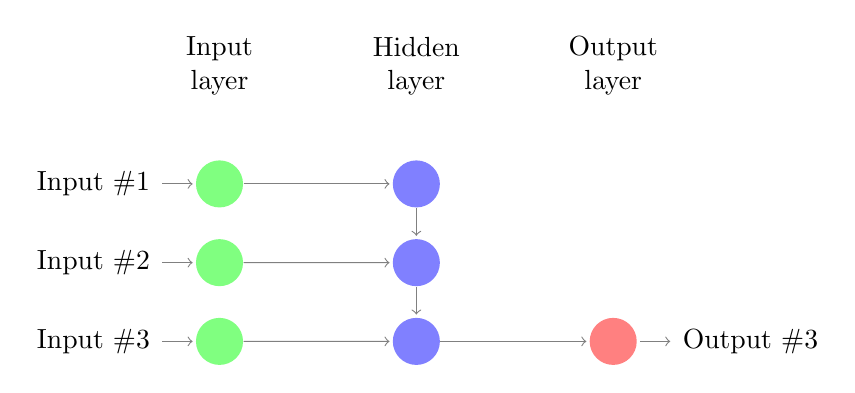
\begin{tikzpicture}[shorten >=1pt,->,draw=black!50, node distance=\layersep]
    \tikzstyle{every pin edge}=[<-,shorten <=1pt]
    \tikzstyle{neuron}=[circle,fill=black!25,minimum size=17pt,inner sep=0pt]
    \tikzstyle{input neuron}=[neuron, fill=green!50];
    \tikzstyle{output neuron}=[neuron, fill=red!50];
    \tikzstyle{hidden neuron}=[neuron, fill=blue!50];
    \tikzstyle{annot} = [text width=4em, text centered]

    % Draw the input layer nodes
    \foreach \name / \y in {1,...,3}
    % This is the same as writing \foreach \name / \y in {1/1,2/2,3/3,4/4}
        \node[input neuron, pin=left:Input \#\y] (I-\name) at (0,-\y) {};

    % Draw the hidden layer nodes
    \foreach \name / \y in {1,...,3}
        \path[yshift=0cm]
            node[hidden neuron] (H-\name) at (\layersep,-\y cm) {};

    \foreach \name / \y in {3,...,3}
    % This is the same as writing \foreach \name / \y in {1/1,2/2,3/3,4/4}
        \node[output neuron,pin={[pin edge={->}]right:Output  \#\y}, right of=H-\y] (O-\y) {};

     % Connect every node in the input layer with every node in the
    % hidden layer.
 
    \foreach \source in {1,...,3}
             \path (I-\source) edge (H-\source);
     \path (H-3) edge (O-3);

     % Connect every node in the hidden layer with the output layer
        
     \path  (H-1) edge    (H-2);
     \path  (H-2) edge    (H-3);

     % Annotate the layers
    \node[annot,above of=H-1, node distance=1.5cm] (hl) {Hidden layer};
    \node[annot,left of=hl] {Input layer};
    \node[annot,right of=hl] {Output layer};
\end{tikzpicture}

   \caption{multi-input single-output Recurrent neural network}
\label{fig:RNNMS}
\end{figure}



\begin{figure}[!h]
\center
\def\layersep{2.5cm}

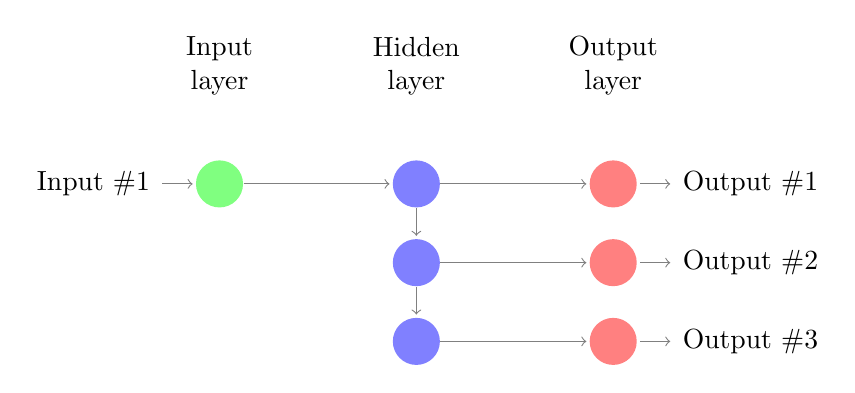
\begin{tikzpicture}[shorten >=1pt,->,draw=black!50, node distance=\layersep]
    \tikzstyle{every pin edge}=[<-,shorten <=1pt]
    \tikzstyle{neuron}=[circle,fill=black!25,minimum size=17pt,inner sep=0pt]
    \tikzstyle{input neuron}=[neuron, fill=green!50];
    \tikzstyle{output neuron}=[neuron, fill=red!50];
    \tikzstyle{hidden neuron}=[neuron, fill=blue!50];
    \tikzstyle{annot} = [text width=4em, text centered]

    % Draw the input layer nodes
    \foreach \name / \y in {1,...,1}
    % This is the same as writing \foreach \name / \y in {1/1,2/2,3/3,4/4}
        \node[input neuron, pin=left:Input \#\y] (I-\name) at (0,-\y) {};

    % Draw the hidden layer nodes
    \foreach \name / \y in {1,...,3}
        \path[yshift=0cm]
            node[hidden neuron] (H-\name) at (\layersep,-\y cm) {};

    \foreach \name / \y in {1,...,3}
    % This is the same as writing \foreach \name / \y in {1/1,2/2,3/3,4/4}
        \node[output neuron,pin={[pin edge={->}]right:Output  \#\y}, right of=H-\y] (O-\y) {};

     % Connect every node in the input layer with every node in the
    % hidden layer.
 
    \foreach \source in {1,...,1}
             \path (I-\source) edge (H-\source);
    \foreach \source in {1,...,3}
             \path (H-\source) edge (O-\source);

     % Connect every node in the hidden layer with the output layer
        
     \path  (H-1) edge    (H-2);
     \path  (H-2) edge    (H-3);

     % Annotate the layers
   \node[annot,above of=H-1, node distance=1.5cm] (hl) {Hidden layer};
   \node[annot,left of=hl] {Input layer};
    \node[annot,right of=hl] {Output layer};
\end{tikzpicture}

   \caption{single-input multi-output Recurrent neural network}
\label{fig:RNNSM}
\end{figure}

\begin{figure}[!h]
\center
\def\layersep{2.5cm}

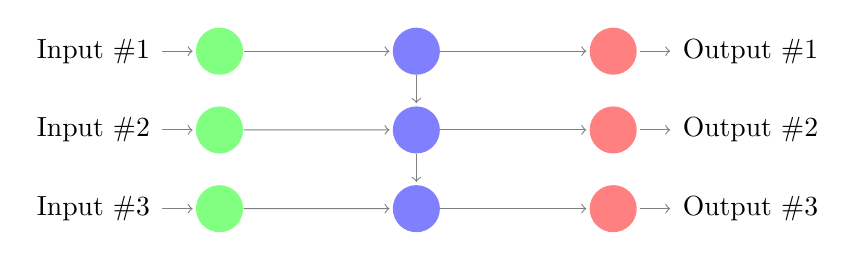
\begin{tikzpicture}[shorten >=1pt,->,draw=black!50, node distance=\layersep]
    \tikzstyle{every pin edge}=[<-,shorten <=1pt]
    \tikzstyle{neuron}=[circle,fill=black!25,minimum size=17pt,inner sep=0pt]
    \tikzstyle{input neuron}=[neuron, fill=green!50];
    \tikzstyle{output neuron}=[neuron, fill=red!50];
    \tikzstyle{hidden neuron}=[neuron, fill=blue!50];
    \tikzstyle{annot} = [text width=4em, text centered]

    % Draw the input layer nodes
    \foreach \name / \y in {1,...,3}
    % This is the same as writing \foreach \name / \y in {1/1,2/2,3/3,4/4}
        \node[input neuron, pin=left:Input \#\y] (I-\name) at (0,-\y) {};

    % Draw the hidden layer nodes
    \foreach \name / \y in {1,...,3}
        \path[yshift=0cm]
            node[hidden neuron] (H-\name) at (\layersep,-\y cm) {};

    \foreach \name / \y in {1,...,3}
    % This is the same as writing \foreach \name / \y in {1/1,2/2,3/3,4/4}
        \node[output neuron,pin={[pin edge={->}]right:Output  \#\y}, right of=H-\y] (O-\y) {};

     % Connect every node in the input layer with every node in the
    % hidden layer.
 
    \foreach \source in {1,...,3}
             \path (I-\source) edge (H-\source);
    \foreach \source in {1,...,3}
             \path (H-\source) edge (O-\source);

     % Connect every node in the hidden layer with the output layer
        
     \path  (H-1) edge    (H-2);
     \path  (H-2) edge    (H-3);

     % Annotate the layers
  %  \node[annot,above of=H-1, node distance=1.5cm] (hl) {Hidden layer};
  %  \node[annot,left of=hl] {Input layer};
   % \node[annot,right of=hl] {Output layer};
\end{tikzpicture}

   \caption{multi-input multi-output Recurrent neural network}
\label{fig:RNNMM}
\end{figure}
\newpage
 

\subsection{Long Short-Term Memory} % (fold)
But recurrent neural networks are difficult to train for a long sequence input, because there are two problems \textbf{"gradient explode"} and \textbf{"gradient vanish"} \cite{pascanu2013difficulty}.  Gradient vanish means that the gradient of the earlier inputs goes exponentially fast towards zero. That make  recurrent neural networks can't learn the long-term dependencies in sequences. Gradient explode means the gradients become exponentially large while training. 
   
   People can change the active function like ReLU to avoid the vanishing gradient problem, but more popular solution is using Long Short-Term Memory which is first invented by Hochreiter and Schmidhuber \cite{hochreiter1997long}.      
   An LSTM memory cell contains self-connected memory cell with its a memory cell, an input gate, an output gate and a forget gate units. LSTM uses a series gate units to control the cell receiving data flow, extracting data flow or forgetting the current state at each time step. 



\begin{figure}[!h]

  \centering

\subfigure[Simple RNN model]{\label{fig:SIS-simple}
\centering
  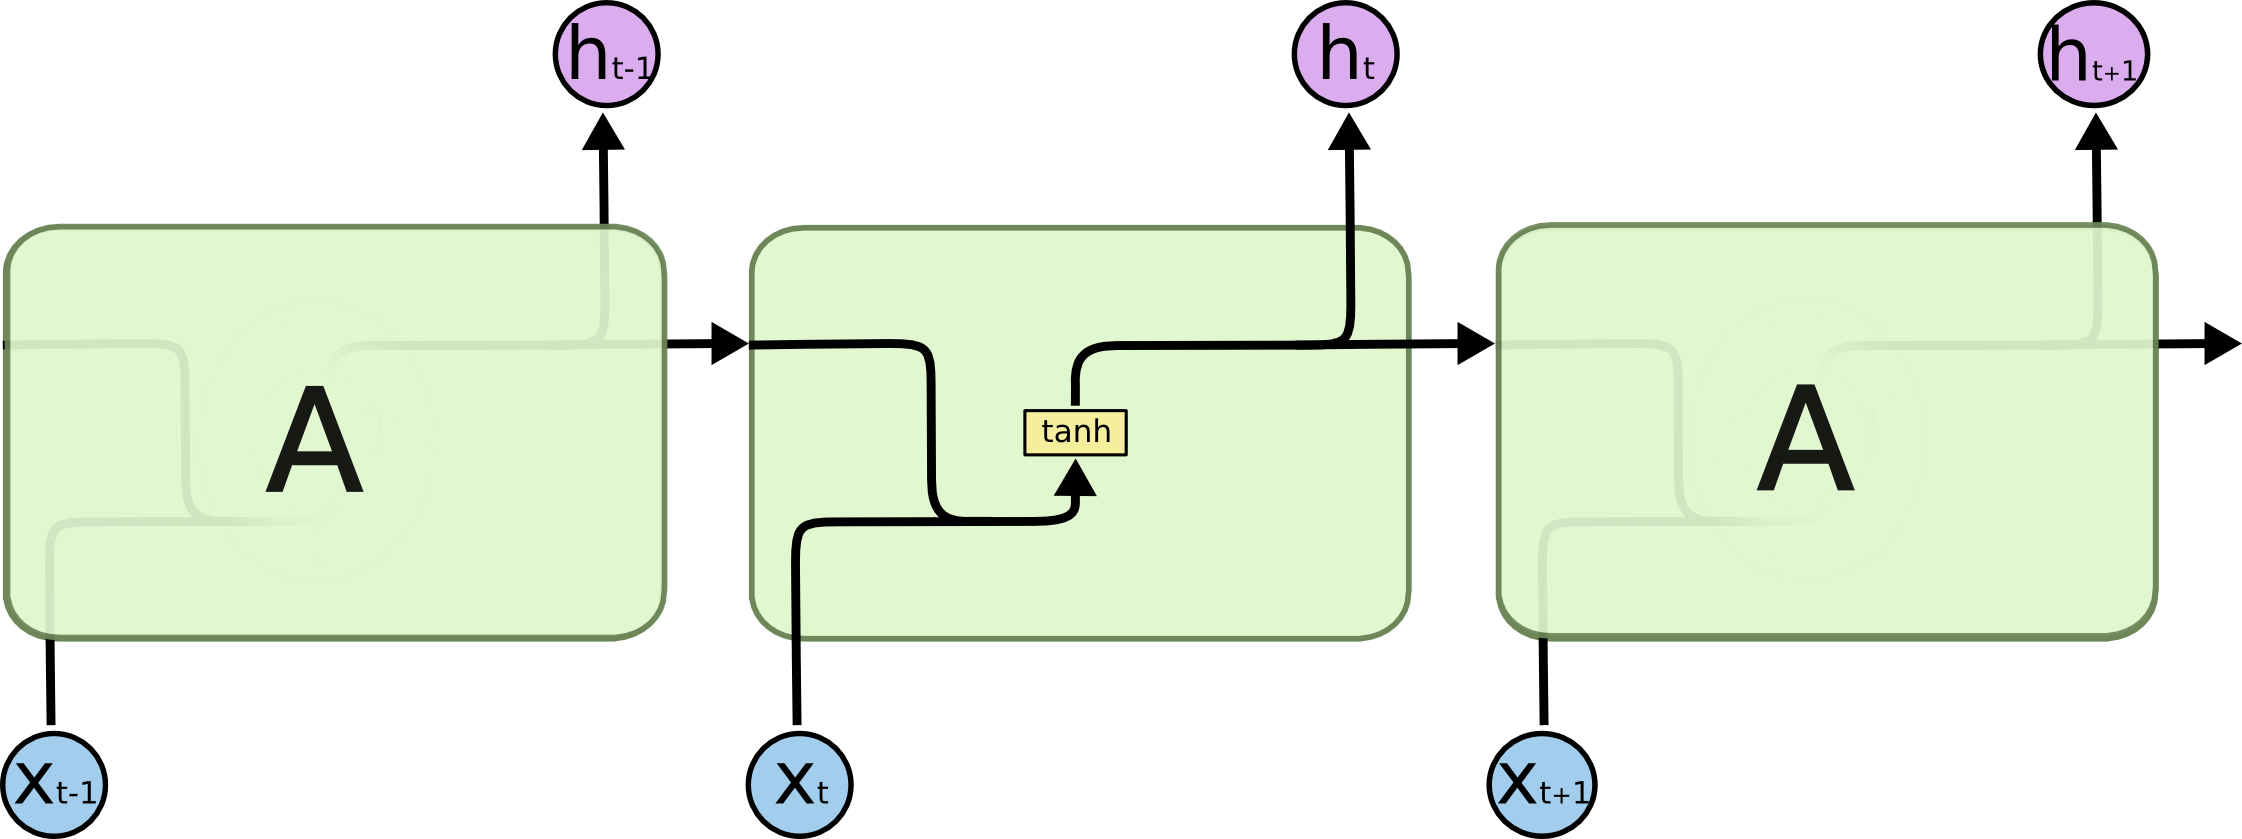
\includegraphics[width=0.48\columnwidth]{images/LSTM3-SimpleRNN.png}
} %
\subfigure[LSTM RNN model]{\label{fig:SIS-LSTM3-chain}
\centering
  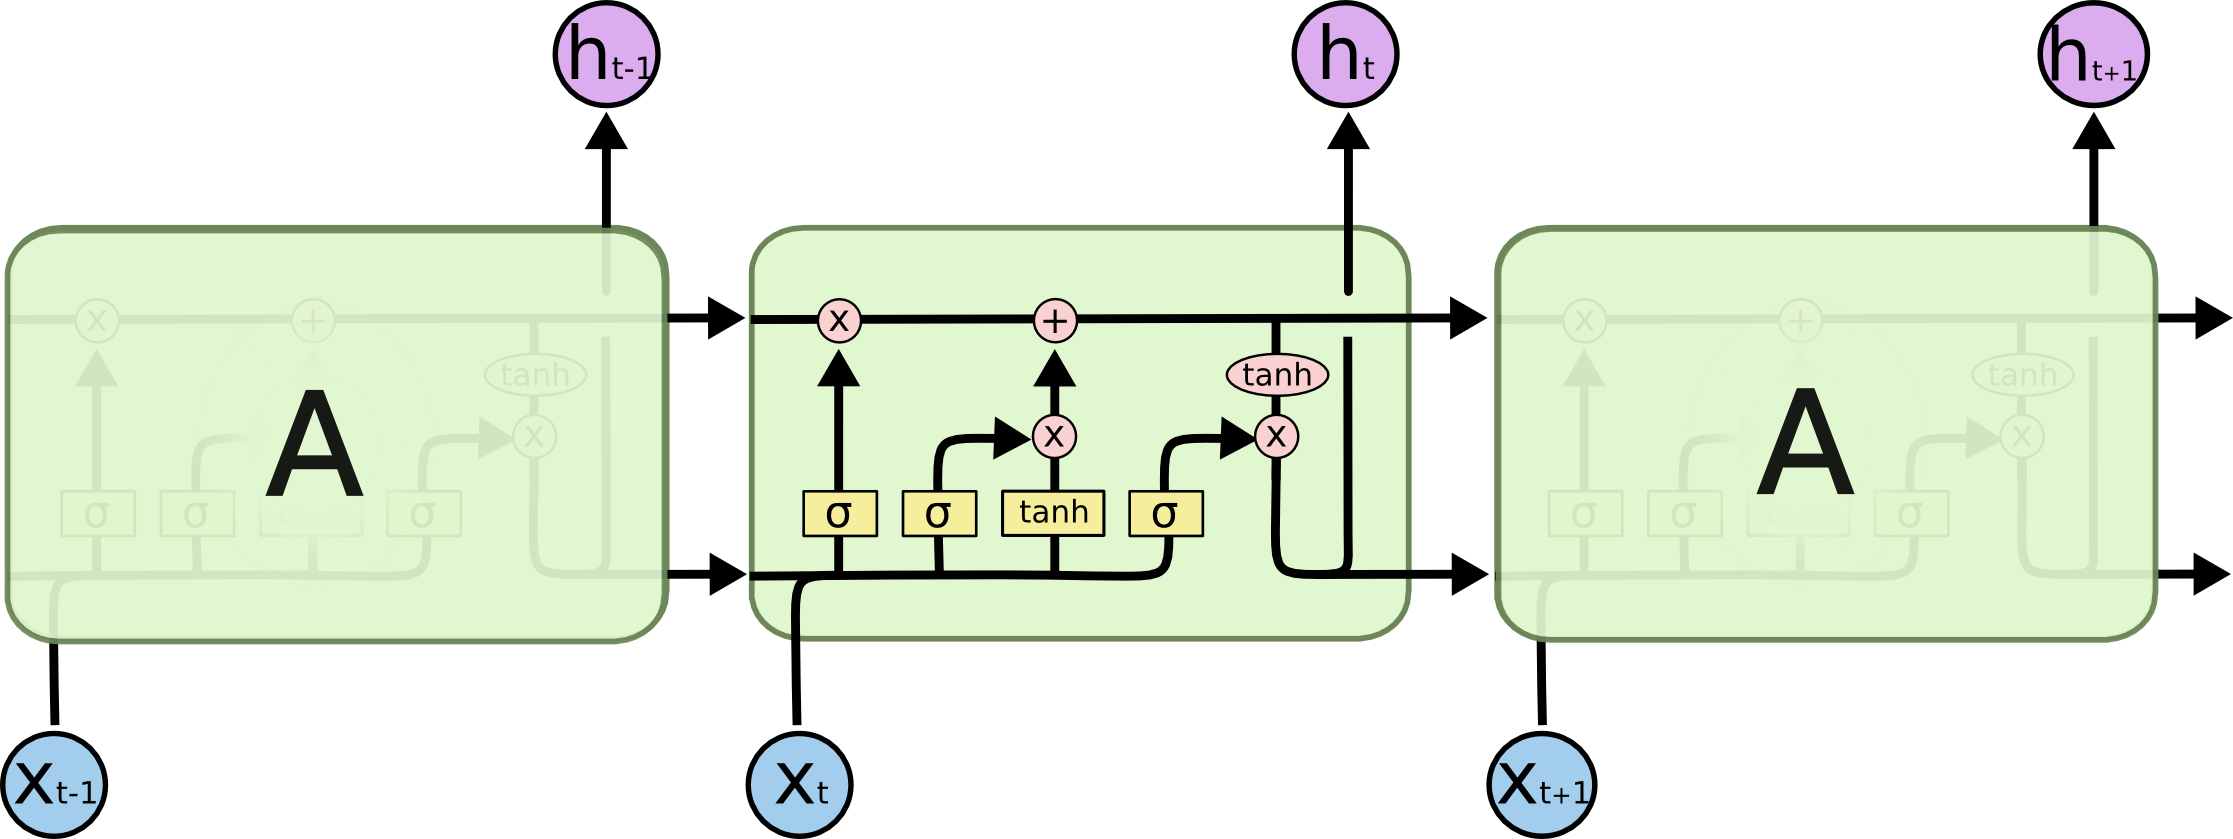
\includegraphics[width=0.48\columnwidth]{images/LSTM3-chain.png}
}

\caption{Two models of RNNs (a) Normal model of RNN with tanh Unit (b) RNN with LSTM Cells (source \cite{olah2015understanding}) }
\label{fig:SISModel}
\end{figure}

\subsection{GRU Cell} % ()
GRU Cell is a special case of LSTM which is invited by  Cho, et al \cite{cho2014learning}.  The forget and input gates are merged into a update gate. The cell state and hidden state are combined as one state. These changes make the structure of GRU simpler than LSTM.

\begin{figure}[!h]
\centering
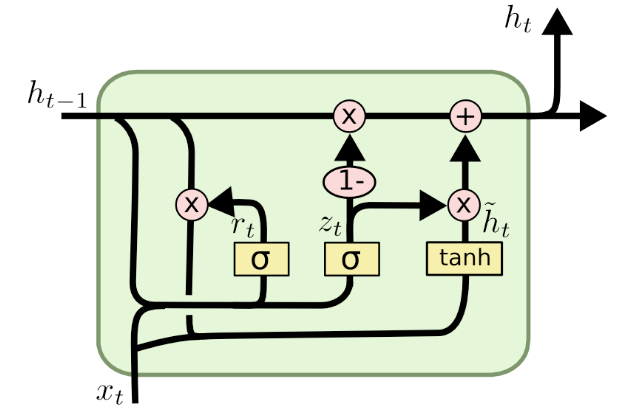
\includegraphics[width=0.55\columnwidth]{images/GRU.png}
\caption{GRU Cell  (source \cite{olah2015understanding})  }
\label{fig:GRU}
\end{figure}

\subsection{Dropout}
To avoid the overfitting we used dropout methode\cite{srivastava2014dropout}. The main idea of dropout is to dropout some units in hidden layer in neural network while training. When training the model some of the units are removed temporarily with probability $p$ as figure \ref{fig:Dropout}.  But while testing the dropout units still join the test. The aim of dropout is to avoid one best state keeping existing, by disabling some units time to time of the network dropout makes the model to be trained in different form every time.  Dropout causes to the convergence speed slower than without it, the model needs more epochs to find the local best solution. But the benefit is it can avoid the overfitting \cite{srivastava2014dropout}. 
\begin{figure}[!h]

  \centering

\subfigure[standard NN model]{\label{fig:NN-simple}
\centering
  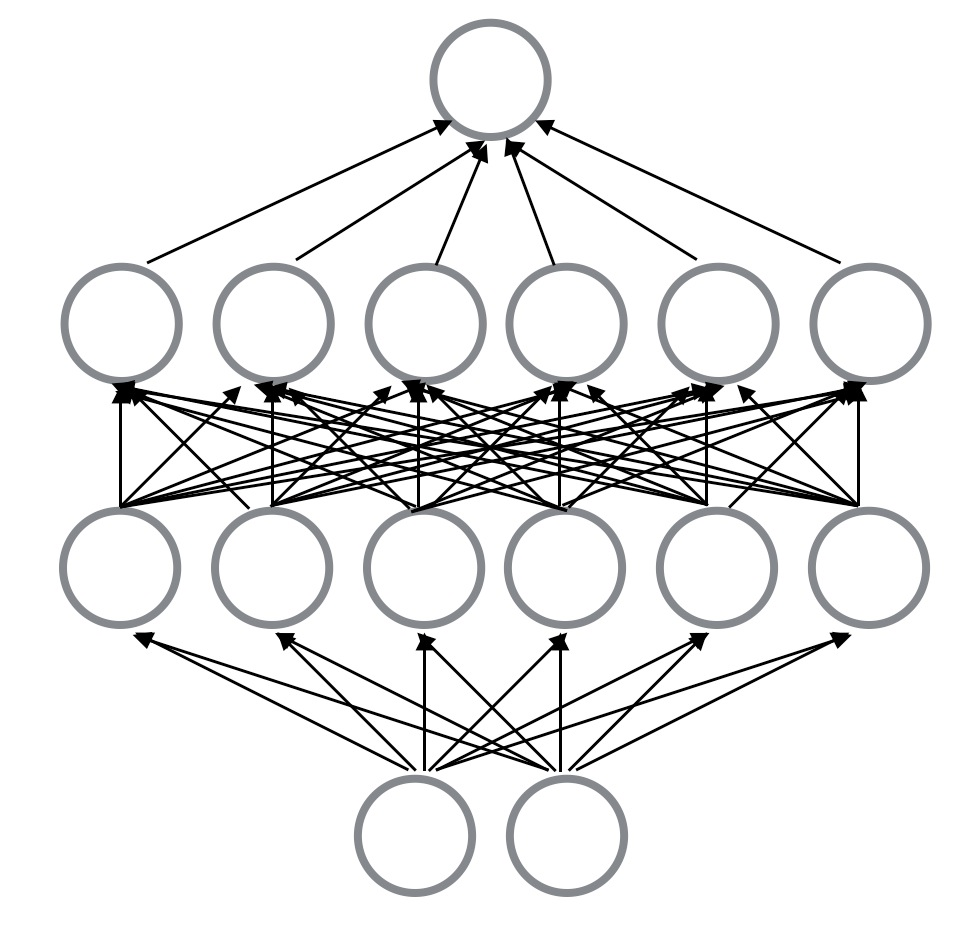
\includegraphics[width=0.48\columnwidth]{images/NNFULL.png}
} %
\subfigure[NN with dropout]{\label{fig:drop}
\centering
  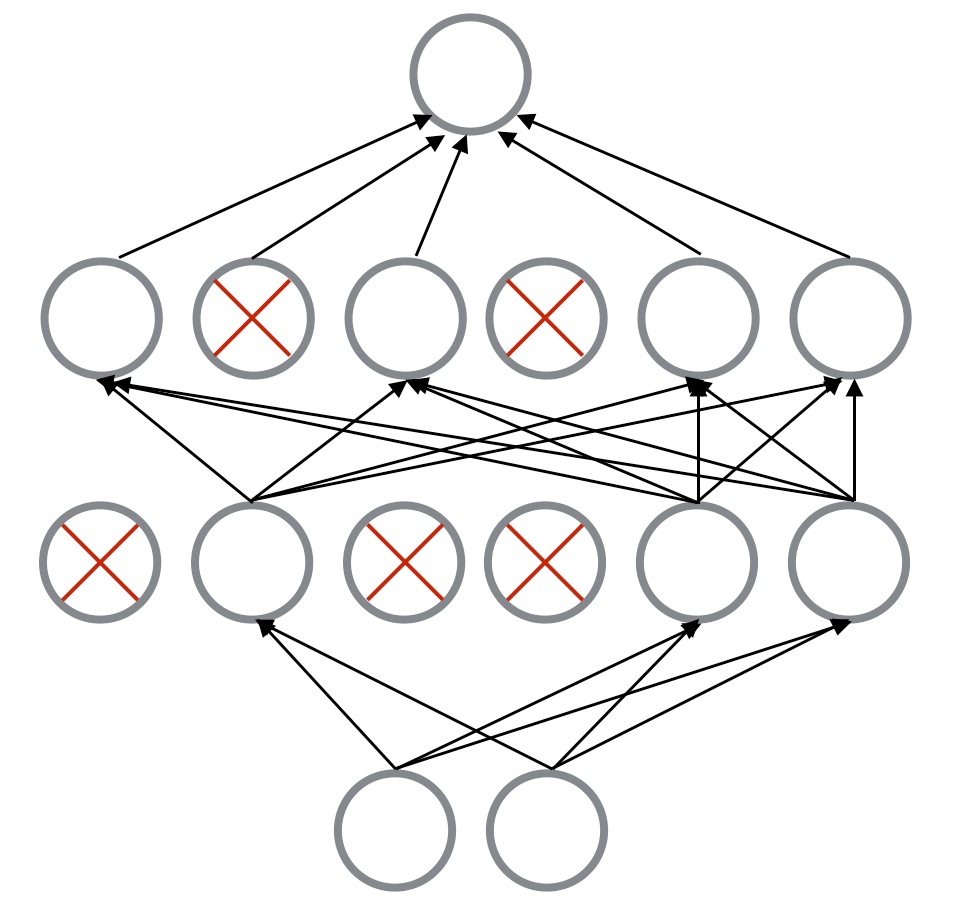
\includegraphics[width=0.48\columnwidth]{images/DROPOUT.png}
}

\caption{Dropout Neural Net Model. (a) a standard neural network (b) after deploying dropout  }
\label{fig:Dropout}
\end{figure}

\newpage
\section{K Fold Cross Validation } 
To limit the overfitting and improve the robustness of the model we often use cross validation technology. K fold cross validation is that the dataset was shuffled and split into k subsets. We train the model with some of subsets and others are used for testing.
\begin{figure}[!h]
\centering
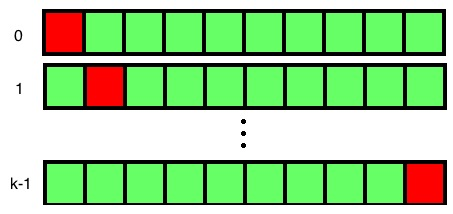
\includegraphics[width=0.55\columnwidth]{images/CrossV.png}
\caption{K Fold Cross Validation (green rectangle is the training set, red rectangle is the testing set)  }
\label{fig:GRU}
\end{figure}

In our work we split the data not equally, we consider an event as a unit.  We use 10 times cross validation, so we split 260 event into 10 subsets. And we test all models with the same shuffled sequence, aka same training sets and test sets.

\section{Levenberg-Marquardt Method} % (fold)
\label{sec:LM}

\section{Spark } % (fold)
\section{Tensorflow } % (fold)

\section{Related Work } % (fold)
People research on Twitter for a long time and there are a lots directions  to study this complex social network like event detection\cite{kimmey2015twitter}, spam detection \cite{ahmed2012mcl} \cite{wang2010don} or sentiment detection\cite{barbosa2010robust}. These work are similar with our task rumor detection but still contain many differences.

People first studied on rumors in psychology area for years \cite{allport1947psychology} \cite{sunstein2014rumors}.
But since Twitter becomes an important platform for people sharing and exchanging information including rumors, the detection of misinformation on twitter turns to be a trending researching topic. 

Researcher first began from studying rumor spreading during several special events like natural disasters\cite{oh2010exploration} \cite{tanaka2012transmission}\cite{mendoza2010twitter}  or terrorist attacks \cite{starbird2014rumors}. But these results are not general enough to other types of rumors. Our data includes sports, politic, entertainment, also natural disasters and other kinds of rumors. 

Carlos Castillo researched the information credibility on Twitter\cite{castillo2011information}\cite{gupta2014tweetcred}. But his work is more about people opinion (trustful or not) to a tweet not the credibility of tweet itself. But it still a good start of resolving problem. Lots of other works are based on Castillo's work \cite{yang2012automatic} \cite{liu2015real} and used different set of features, for example yang \cite{yang2012automatic} add the location of poster and the client type of user (web client or mobile phone) as two important features.
And 



There are rencent researches based on the propagation structure of rumor on Sina Weibo\cite{wu2015false}  \cite{bao2013new}, but Twitter doesn't give us such detail of propagation like Weibo, so these works are useless for us. 

Liu's work \cite{wu2015false} focused on one type of rumor "the false photos" on social network not the general type of rumors.  

Xiaomo claimed their system is the first real time rumor debunking system on Twitter \cite{liu2015real}. But their work are similar with above other previous works, they use the static features of rumors and ignored the feature's changing over time during the event spreading on the social network which can be seen in figure \ref{fig:Url5000} and \ref{fig:largecity}. The fraction of tweets containing url with top 5000 domain and the fraction of poster living in large city which are both constantly changing. But one feature called "crowd wisdom" is an new idea and we use it in our work.

\begin{figure}[!h]
\centering
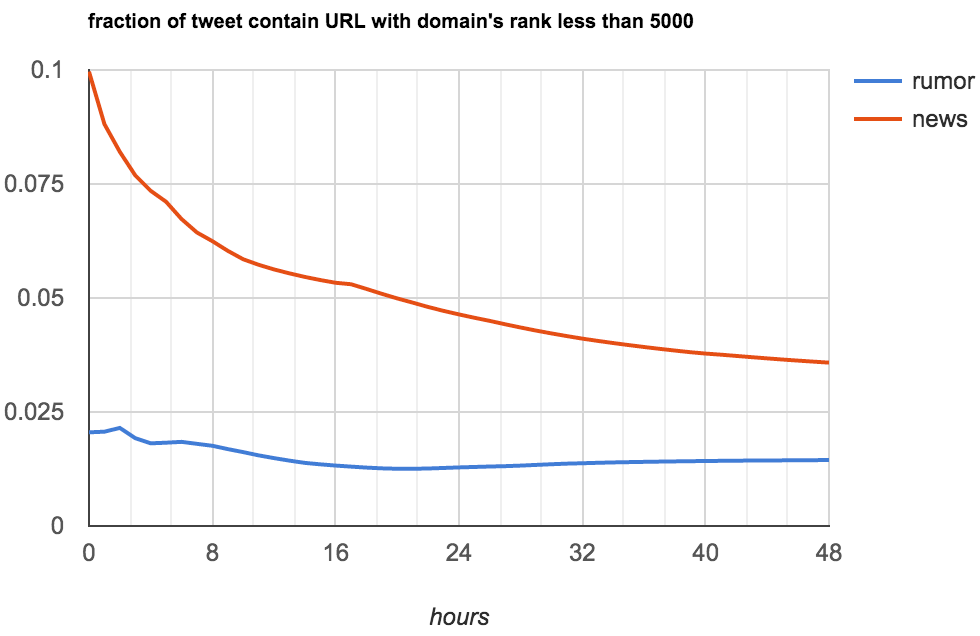
\includegraphics[width=0.52\columnwidth]{images/url5000.png}
\caption{The fraction of tweets containing url with top 5000 domain}
\label{fig:Url5000}
\end{figure}
\begin{figure}[!h]
\centering
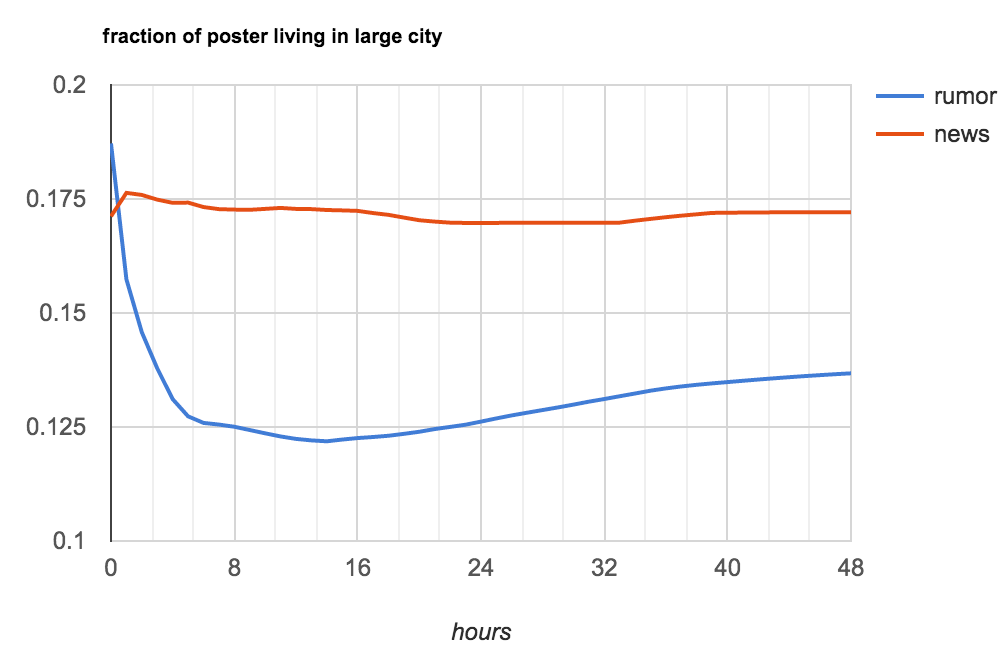
\includegraphics[width=0.52\columnwidth]{images/largecity.png}
\caption{The fraction of poster living in large city}
\label{fig:largecity}
\end{figure}

\newpage
Other researchers used propagation models like SpikeM \cite{kwon2013prominent} and SEIZ models \cite{jin2013epidemiological} to capture the tweet's volume changing over time, but they didn't use other features into time series model. And these features can't show the effect in the early stage of rumor spreading. We can provide it in the later section \ref{featureanalyzing}.

J Ma used Recurrent Neural Networks for rumor detection \cite{madetecting}, as the same disadvantage of the other Neural Networks models, the process of model's training is black box to us, so we can't know way we got this result. In our case we can't get the evidences to convince people why the detected event is more likely to be a rumor or rather than a breaking news. 

Another work from J Ma used a time series model called Dynamic Series-Time Structure \cite{ma2015detect} to capture the variation of features. But they only used the features of social content and they didn't further explain how the performances of features change over time or how do they improve the performance of the model in first few hours after the events beginning.  We use their Series-Time Structure with our extended data and we will show how do these features change during time.

